% 使用ctexart文档类(用XeLaTeX编译,直接支持中文)
\documentclass{ctexart}

% 导言区,可以在此引入必要的宏包
\usepackage{pgf-umlcd}
\usepackage{csquotes}

\begin{document} %在document环境中撰写文档
  \begin{figure}[!htp]
  \centering
  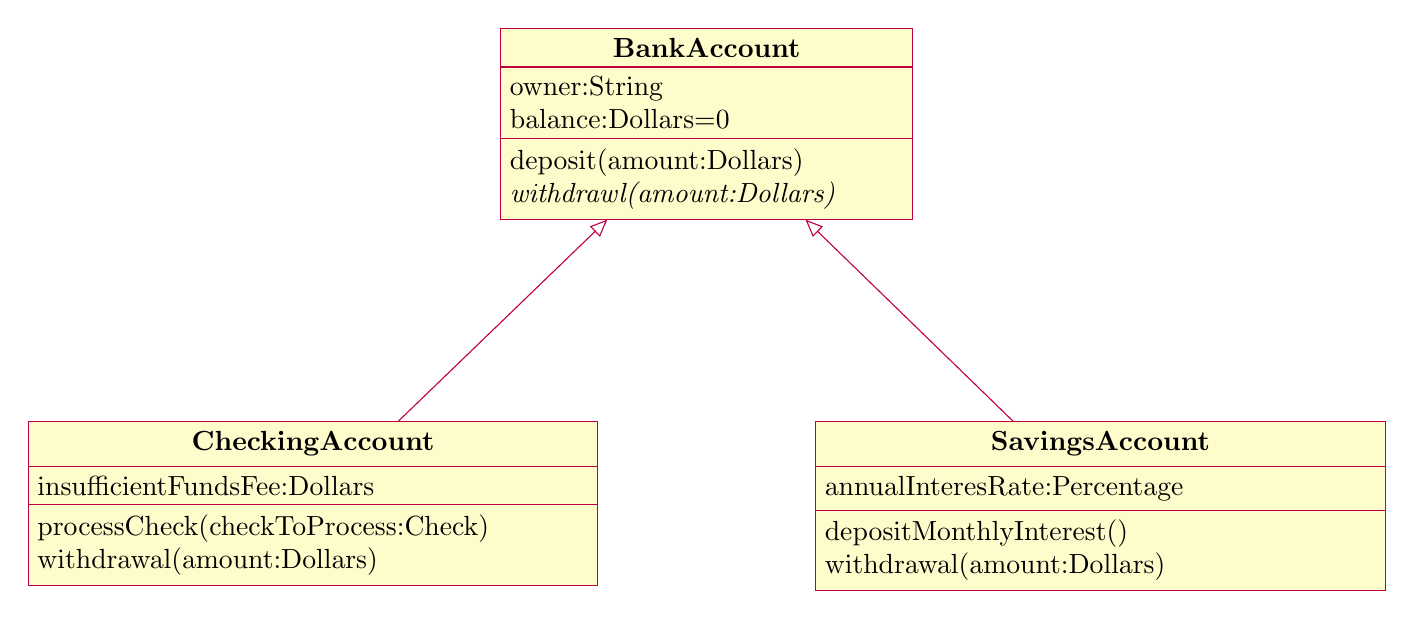
\begin{tikzpicture}
    \begin{class}[text width=5cm]{BankAccount}{0,0}
      \attribute{owner:String}
      \attribute{balance:Dollars=0}
      \operation{deposit(amount:Dollars)}
      \operation[0]{withdrawl(amount:Dollars)}
    \end{class}
    \begin{class}[text width=7cm]{CheckingAccount}{-5,-5}
      \inherit{BankAccount}
      \attribute{insufficientFundsFee:Dollars}
      \operation{processCheck(checkToProcess:Check)}
      \operation{withdrawal(amount:Dollars)}
    \end{class}
    \begin{class}[text width=7cm]{SavingsAccount}{5,-5}
      \inherit{BankAccount}
      \attribute{annualInteresRate:Percentage}
      \operation{depositMonthlyInterest()}
      \operation{withdrawal(amount:Dollars)}
    \end{class}
  \end{tikzpicture}
  \caption{用\enquote{pgf-umlcd}宏包绘制UML图}\label{fig:uml}
\end{figure}

\begin{figure}[!hpt]
  \centering
  \begin{tikzpicture}[font=\small, show background grid]
    \tikzset{ coord/.style={coordinate} }    
    \begin{class}[fill=red!25, text width=4em]{动物类CAnimal}{0, 0}
      \attribute{-name[32]:char}
      \attribute{-age:int}
      \attribute{-weight:int}
      \operation{+show():void}
    \end{class}

    \begin{class}[fill=green!25, text width=4em]{马CHorse}{-3, -2.5}
      \inherit{动物类CAnimal}
      \attribute{-power:int}
      \operation{+show():void}
      \operation{+talk():void}
    \end{class}
      
    \begin{class}[fill=green!25, text width=4em]{鸟CBird}{0, -2.5}
      \inherit{动物类CAnimal}
      \attribute{-wingSpan:int}
      \operation{+show():void}
      \operation{+talk():void}
    \end{class}
      
    \begin{class}[fill=green!25, text width=4em]{牛CBull}{3, -2.5}
      \inherit{动物类CAnimal}
      \attribute{-power:int}
      \operation{+show():void}
      \operation{+talk():void}
    \end{class}

    \begin{class}[fill=blue!25, text width=4em]{飞马CPegasus}{-1.5, -5}
      \inherit{马CHorse}
      \inherit{鸟CBird}
      \operation{+show():void}
      \operation{+talk():void}
    \end{class}           
  \end{tikzpicture}  
  \caption{test}
  \label{test}
\end{figure}
\end{document}

%%% Local Variables:
%%% mode: latex
%%% TeX-master: t
%%% End:
